\documentclass{standalone}
\usepackage{tikz}
\usepackage{helvet}
\usetikzlibrary{arrows.meta}
\usetikzlibrary{decorations.pathreplacing}
\usepackage{varwidth}
\usetikzlibrary{fit}

\begin{document}
    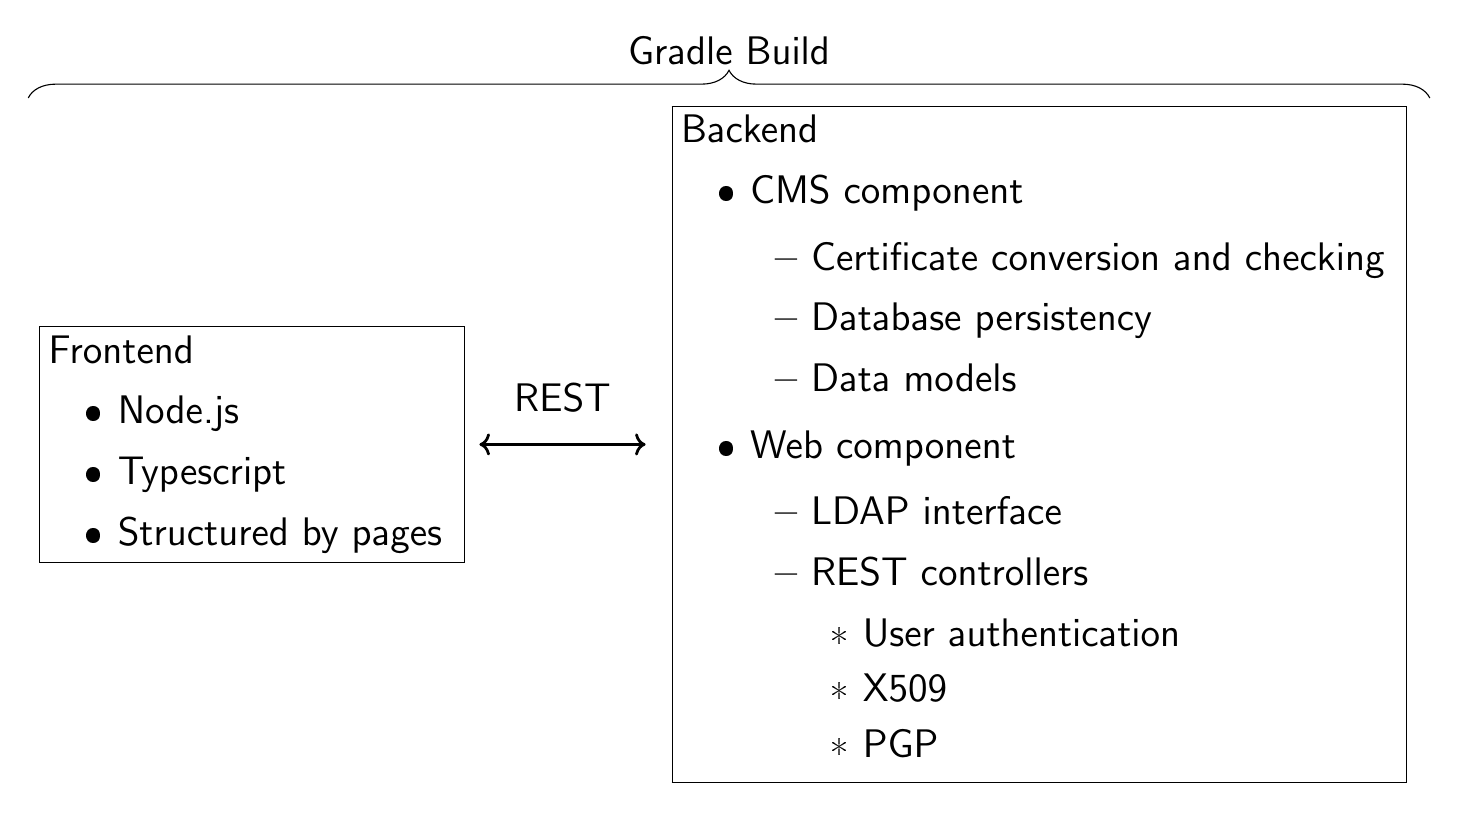
\begin{tikzpicture}[font=\sffamily\small]
        \draw [decorate,decoration={brace,amplitude=10pt},xshift=-4pt,yshift=0pt] (-2.7,4.4) -- (15.1,4.4)
        node [black,midway,yshift=0.6cm] {\Large Gradle Build};
        \node at (0, 0) {\framebox{\Large
        {\begin{varwidth}{\linewidth}
             Frontend
             \begin{itemize}
                 \item Node.js
                 \item Typescript
                 \item Structured by pages
             \end{itemize}
        \end{varwidth}}
        }};
        \draw [<->,line width=1pt] (2.89, 0) -- (5, 0)
        node [black,midway,yshift=0.6cm] {\Large REST};
        \node at (10, 0) {\framebox{\Large
        {\begin{varwidth}{\linewidth}
             Backend
             \begin{itemize}
                 \item CMS component
                 \begin{itemize}
                     \item Certificate conversion and checking
                     \item Database persistency
                     \item Data models
                 \end{itemize}
                 \item Web component
                 \begin{itemize}
                     \item LDAP interface
                     \item REST controllers
                     \begin{itemize}
                         \item User authentication
                         \item X509
                         \item PGP
                     \end{itemize}
                 \end{itemize}
             \end{itemize}
        \end{varwidth}}
        }};
    \end{tikzpicture}
\end{document}
